\documentclass{article}
\usepackage{hyperref}
\usepackage{graphicx}
\usepackage{listings}

\title{INFO-F-311: Artificial Intelligence - Project 1: Search}
\author{Bourgeois Noé}
\date{2023 October 8}

\begin{document}

\maketitle

\tableofcontents

\newpage
\section{Introduction}
This report outlines the solution of problem trough 
the implementation of artificial intelligence techniques 
based on graph search.

For references, please refer to the project instructions.

\section{Results}
\subsection{Paths Sizes and Nodes Expansions Comparison}
Comparison of the number of nodes expanded in BFS, DFS, and A* during the solution of level 3 and the final path sizes

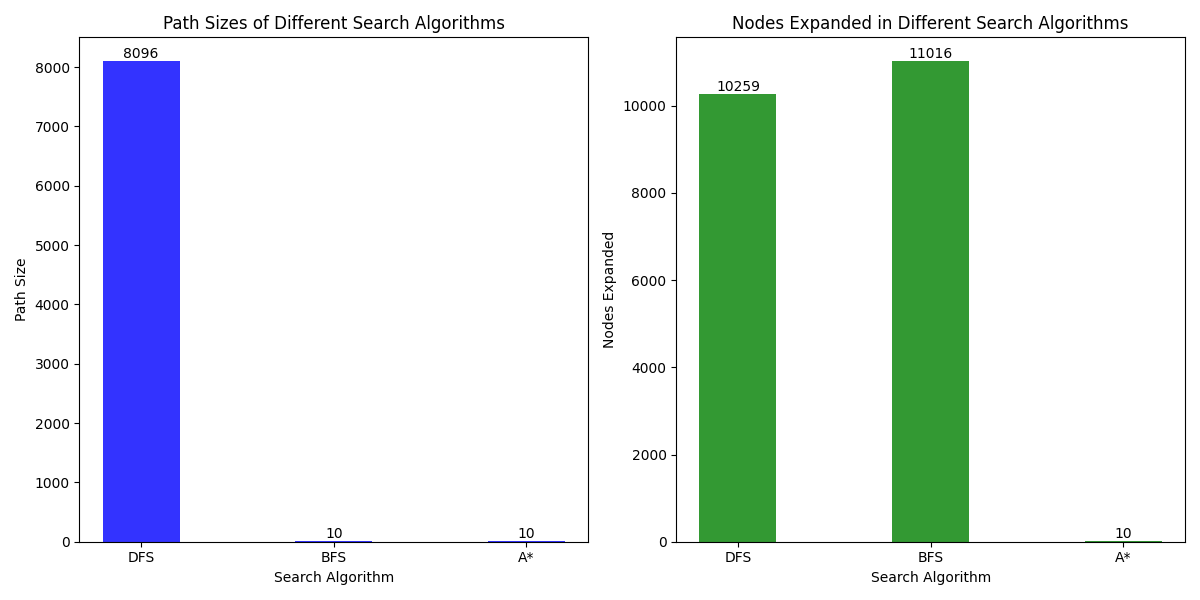
\includegraphics[width=\textwidth]{media/Figure_1.png}


% \begin{tabular}{|c|c|c|c|}
%     \hline
%     Algorithm & Path Size & Nodes Expanded \\
%     \hline
%     DFS & 8096 & 10259 \\
%     BFS & 10 & 11016 \\
%     A* & 10 & 10 \\
%     \hline
% \end{tabular}

\subsection{Discussion}
\begin{itemize}
    \item \textbf{Efficiency}: A* is the most efficient in terms of both path size and nodes expanded.
    \item \textbf{Optimality}: BFS and A* find the optimal path, while DFS does not.
    \item \textbf{Resource Usage}: DFS and BFS are resource-intensive, whereas A* is memory-efficient.
    \item \textbf{Applicability}: A* is often the best choice when an admissible heuristic is available.
    \item \textbf{Path Quality}: DFS finds a path but a horrible one.
\end{itemize}    

\section{Heuristics Development}

    The heuristics for both the \textit{CornerSearchProblem} and the \textit{GemSearchProblem} share a common foundation. 
    Essentially, both problems can be reduced to a form of the Traveling Salesman Problem (TSP) for multi-agent systems. 
    
    \subsection{Common Foundation: Multi-Agent TSP}
    The fundamental problem for both corner and gem scenarios is to 
    find the shortest possible route that visits a set of target locations (corners or gems) 
    and finishes to an exit point. This is akin to the TSP with multiple agents involved. 

    The heuristic employs a greedy approach, 
    where agents iteratively move to the Manhattan distance nearest unvisited objective. 
    After all objectives are visited, agents proceed to the nearest exit. 
    The total distance traveled serves as the heuristic value.

    \subsection{Optimization}
    The TSP currently searches the shortest paths only among the start and objective positions.
    Including the exit positions would make the search complete, but as it adds a deterministic end 
    extremity to the paths it also increases the computation time and memory usage so we decided to not include them.
    As objectives position are given with the problem's world map, 
    both heuristics can be further optimized using techniques like memoization, 
    and pre-computation of distances between key points, thereby making the algorithm more efficient.

\section{ChatGPT Usage}
\subsection{Data Dump}
In the initial stage, I fed ChatGPT with as much contextual information as possible. 
\begin{itemize}
    \item project instructions
    \item State of the art
    \item my related work
\end{itemize}

\subsubsection{Memory}
The project leverages extended memory capabilities through the use of text files, Microsoft Word documents, and other data storage formats. These files serve as a contextual database for the ChatGPT tool. 

\begin{itemize}
    \item \textbf{Extended Memory}: Storing information in these external files provides a form of "extended memory" for GPT, which enables the model to access a wider context than its built-in limitations.
    \item \textbf{Dynamic Updates}: As new information becomes available, whether from personal learnings, friends, teachers, or Q\&A sessions, these files are updated to reflect the latest knowledge and insights.
    \item \textbf{Efficiency}: This approach minimizes the need for repetitive instruction to GPT, thereby making the process more efficient.
\end{itemize}
\subsection{Filtering Output}
ChatGPT's output also underwent a filtration process to distill the most useful and relevant suggestions or solutions. 
This step ensured that the AI's contributions were directly applicable to the project.

\end{document}
